\section{LVish, formally}\label{s:quasi-formal}

In this section, \either{I}{we} present $\lambdaLVish$, a core calculus for the
LVish programming model. It extends the $\lambdaLVar$ language of
\either{Chapter}{Section}~\ref{ch:lvars}. Rather than
modeling the full ensemble of event handlers, handler pools,
quiescence, and freezing as separate primitives in $\lambdaLVish$, though,
\either{I}{we} instead formalize
the ``freeze-after'' pattern---which combined them---directly as a
primitive.  This simplifies the calculus while still capturing the
essence of the programming model.  \either{I}{We} also generalize the @put@
operation to allow the arbitrary \emph{update operations} of Section~\either{\ref{subsection:lvars-generalizing-from-least-upper-bound-writes}}{\ref{s:lvars-generalizing}},
which are inflationary and commutative but do not necessarily compute
a lub.

\subsection{Freezing}

To model freezing, we need to generalize the notion of the state of an
LVar to include information about whether it is ``frozen'' or not.
Thus, in $\lambdaLVish$ an LVar's \emph{state} is a pair
$\state{d}{\status}$, where $d$ is an element of the set $D$ and $\status$ is a ``status bit'' of
either $\frozentrue$ or $\frozenfalse$.  A state where $\status$ is
$\frozenfalse$ is ``unfrozen'', and one where $\status$ is
$\frozentrue$ is ``frozen''.

\either{I}{We} define an ordering $\leqp$ on LVar states $\state{d}{\status}$ in
terms of the given ordering $\userleq$ on elements of
$D$.  Every element of $D$ is ``freezable'' except $\top$.
Informally:
\begin{itemize}
\item Two unfrozen states are ordered according to the
  given $\userleq$; that is, $\state{d}{\frozenfalse}
  \leqp \state{d'}{\frozenfalse}$ exactly when $d \userleq d'$.
\item Two frozen states do not have an order, unless they are equal:
  $\state{d}{\frozentrue} \leqp \state{d'}{\frozentrue}$ exactly when
  $d = d'$.
\item An unfrozen state $\state{d}{\frozenfalse}$ is less than or
  equal to a frozen state $\state{d'}{\frozentrue}$ exactly when $d
  \userleq d'$.
\item The only situation in which a frozen state is less than an
  unfrozen state is if the unfrozen state is $\top$; that is,
  $\state{d}{\frozentrue} \leqp \state{d'}{\frozenfalse}$ exactly when
  $d' = \top$.
\end{itemize}
Adding status bits to each element (except $\top$) of the lattice $(D,
\userleq, \bot, \top)$ results in a new lattice $(D_p, \leqp, \botp,
\topp)$.  (The $p$ stands for pair, since elements of this new lattice
are pairs $\state{d}{\status}$.) \either{I}{We} write $\lubp{}{}$ for the lub
operation that $\leqp$ induces.
Definitions~\ref{def:lattice-with-status-bits} and \ref{def:lubp} and
Lemmas~\ref{lem:partition-of-Dp} and~\ref{lem:lattice-structure}
formalize this notion.
\ifdefined\JOURNAL
As before, we only give the statements of the lemmas here; the proofs
appear in~\cite{lvars-dissertation}.
\fi

\DefLatticeWithStatusBits

\LemPartitionOfDp
\ifdefined\DISSERTATION
\begin{proof}
  Immediate from Definition~\ref{def:lattice-with-status-bits}.
\end{proof}
\fi

\DefLubP

Lemma~\ref{lem:lattice-structure} says that if $(D, \leq, \bot, \top)$
is a lattice, then $(D_p, \leqp, \botp, \topp)$ is as well:

\LemLatticeStructure
\ifdefined\DISSERTATION
\begin{proof}
See Section~\ref{section:lattice-structure-proof}.
\end{proof}
\fi

\subsection{Update operations}\label{subsection:quasi-update-operations}

$\lambdaLVish$ generalizes the @put@ operation of $\lambdaLVar$ to a
family of operations $\PUTi$, in order to allow the generalized update
operations of
Section~\either{\ref{subsection:lvars-generalizing-from-least-upper-bound-writes}}{\ref{s:lvars-generalizing}}
that are commutative and inflationary, but do not necessarily compute
a lub.  To make this possible we parameterize $\lambdaLVish$ not only
by the lattice $(D, \userleq, \bot, \top)$, but also by a set $U$ of
\emph{update operations}, as discussed previously in
Section~\either{\ref{subsection:lvars-generalizing-from-least-upper-bound-writes}}{\ref{s:lvars-generalizing}}:

\DefSetOfUpdateOperations

\noindent The first of the conditions in
Definition~\ref{def:set-of-update-operations} says that each update
operation is inflationary with respect to $\userleq$, and the second
condition says that update operations commute with each other.  Every
set of update operations always implicitly contains the identity
function.

If we want to recover the original semantics of @put@,
we can do so by instantiating $U$ such that there is one
$u_i$ for each element $d_i$ of the lattice $D$, and defining $u_i(d)$
to be $\userlub{d}{d_i}$.  On the other hand, if $D$ is a lattice of
natural numbers and we want increment-only counters, we can
instantiate $U$ to be a singleton set $\setof{ u }$ where $u(d) = d +
1$.  (As described in
Section~\either{\ref{subsection:lvars-generalizing-from-least-upper-bound-writes}}{\ref{s:lvars-generalizing}},
we could also have a set of update operations $\{ u_{(+1)}, u_{(+2)},
\dots \}$, where $u_{(+1)}(d)$ increments $d$'s contents by one,
$u_{(+2)}(d)$ increments by two, and so on.) Update operations are
therefore general enough to express lub writes as well as
non-idempotent increments.  (When a write is specifically a lub write,
\either{I}{we} will continue to use the notation @put@, without the subscript.)

In $\lambdaLVar$, the @put@ operation took two arguments, a location
$l$ and a lattice element $d$.  The $\PUTi$ operations take a location
$l$ as their only argument, and $\putiexp{l}$ performs the update
operation $u_i(l)$ on the contents of $l$.

More specifically, since $l$ points to a state $\state{d}{\status}$
instead of an element $d$, $\putiexp{l}$ must perform $u_{p_i}$, a
lifted version of $u_i$ that applies to states.  Given $U$, we define
the set $U_p$ of lifted operations as follows:

\DefSetOfStateUpdateOperations

\noindent Because every set $U$ of update operations implicitly contains the
identity function, the same is true for the set $U_p$ of state update
operations.  Furthermore, it is easy to show that state update
operations commute, just as update operations do; that is, $\forall d,
i, j.  \;\; u_{p_i}(u_{p_j}(p)) = u_{p_j}(u_{p_i}(p))$.

\lk{I've done the proof of this, but I'm not including it here because
  it seems pretty obvious from the definition.}

\subsection{Stores}

During the evaluation of $\lambdaLVish$ programs, a \emph{store} $S$
keeps track of the states of LVars.  Each LVar is represented by a
binding from a location $l$, drawn from a set $\Loc$, to its state,
which is some pair $\state{d}{\status}$ from the set $D_p$.  The way
that stores are handled in $\lambdaLVish$ is very similar to how they
are handled in $\lambdaLVar$, except that store bindings now point to
states $\state{d}{\status}$, that is, elements of $D_p$, instead of
merely to $d$, that is, elements of $D$.

\DefStore

\either{I}{We} use the notation $\extS{S}{l}{d}{\status}$ to denote extending $S$
with a binding from $l$ to $\state{d}{\status}$.  If $l \in \dom{S}$,
then $\extS{S}{l}{d}{\status}$ denotes an update to the existing
binding for $l$, rather than an extension.  Another way to denote a
store is by explicitly writing out all its bindings, using the
notation $\store{\storebinding{l_1}{d_1}{\status_1},
  \storebinding{l_2}{d_2}{\status_2}, \dots}$.

We can lift the $\leqp$ and $\lubp{}{}$ operations defined on elements
of $D_p$ to the level of stores:

\DefLeqStore

\DefLubStore

If, for example,
\[ \lubp{\state{d_1}{\status_1}}{\state{d_2}{\status_2}} = \topp, \]
then
\[ \lubstore{\store{\storebinding{l}{d_1}{\status_1}}}{\store{\storebinding{l}{d_2}{\status_2}}} =
\topS. \]

\noindent Just as a store containing a binding $\storebindingRaw{l}{\top}$ can
never arise during the execution of a $\lambdaLVar$ program, a store
containing a binding $\storebinding{l}{\top}{\status}$ can never arise
during the execution of a $\lambdaLVish$ program. An attempted write
that would take the value of $l$ to
$\state{\top}{\frozenfalse}$---that is, $\topp$---will raise an error,
and there is no $\state{\top}{\frozentrue}$ element of $D_p$.

\subsection{$\lambdaLVish$: syntax and semantics}

The syntax of $\lambdaLVish$ appears in
Figure~\ref{f:lambdaLVish-syntax}, and
Figures~\ref{f:lambdaLVish-reduction-semantics}
and~\ref{f:lambdaLVish-context-semantics} together give the
operational semantics.  As with $\lambdaLVar$ in
\either{Chapter}{Section}~\ref{ch:lvars}, both the syntax and semantics are
parameterized by the lattice $(D, \userleq, \bot, \top)$, and the
operational semantics is split into two parts, a \emph{reduction
  semantics}, shown in
Figure~\ref{f:lvars-lambdaLVar-reduction-semantics}, and a
\emph{context semantics}, shown in
Figure~\ref{f:lvars-lambdaLVar-context-semantics}.  The reduction
semantics is also parameterized by the set $U$ of update operations.

\FigLambdaLVishGrammar

The $\lambdaLVish$ grammar has most of the expression forms of
$\lambdaLVar$: variables, values, application expressions, @get@
expressions, and @new@.  Instead of @put@ expressions, it has $\PUTi$
expressions, which are the interface to the specified set of update
operations.  $\lambdaLVish$ also adds two new language forms, the
@freeze@ expression and the $\FAW$ expression, which \either{I}{we} discuss in more
detail below.

Values in $\lambdaLVish$ include all those from $\lambdaLVar$---the
unit value $\unit$, lattice elements $d$, locations $l$, threshold
sets $P$, and $\lambda$ expressions---as well as states $p$, which are
pairs $\state{d}{\status}$, and event sets $Q$.  Instead of $T$, \either{I}{we} now
use the metavariable $P$ for threshold sets, in keeping with the fact
that in $\lambdaLVish$, members of threshold sets are states $p$.

As with $\lambdaLVar$, the $\lambdaLVish$ context relation
$\ctxstepsto$ has only one rule, {\sc E-Eval-Ctxt}, which allows us to
apply reductions within a context. The rule itself is identical to the
corresponding rule in $\lambdaLVar$, although the set of evaluation
contexts that the metavariable $E$ ranges over is different.

\FigLambdaLVishReductionSemantics

\FigLambdaLVishContextSemantics

\subsection{Semantics of \il{new}, $\PUTi$, and \il{get}}\label{subsection:quasi-semantics-of-new-put-and-get}

Because of the addition of status bits to the semantics, the {\sc
  E-New} and {\sc E-Get} rules have changed slightly from their
counterparts in $\lambdaLVar$:

\begin{itemize}
\item @new@ (implemented by the {\sc E-New} rule) extends the store
  with a binding for a new LVar whose initial state is $(\bot,
  \frozenfalse)$, and returns the location $l$ of that LVar (\ie, a
  pointer to the LVar).
\item @get@ (implemented by the {\sc E-Get} rule) performs a blocking
  threshold read.  It takes a pointer to an LVar and a threshold
    set $P$, which is a non-empty set of LVar states that must be
  pairwise incompatible, expressed by the premise $\incomp{P}$.
  A threshold set $P$ is pairwise incompatible iff the lub of any two
  distinct elements in $P$ is $\topp$.  If the LVar's state $p_1$ in
  the lattice is at or above some $p_2 \in P$, the @get@
  operation unblocks and returns $p_2$.
\end{itemize}

\noindent $\lambdaLVish$ replaces the $\lambdaLVar$ @put@ operation with the $\PUTi$
operation, which is actually a set of operations that are the interface
to the provided update operations $u_i$.  For each update
operation $u_i$, $\PUTi$ (implemented by the {\sc E-Put} rule) takes a
pointer to an LVar and updates the LVar's state to the result of calling
$u_{p_i}$ on the LVar's current state, potentially pushing the state
of the LVar upward in the lattice.  The {\sc E-Put-Err} rule applies
when a $\PUTi$ operation would take the state of an LVar to $\topp$;
in that case, the semantics steps to $\error$.

\subsection{Freezing and the $\FAW$ primitive}\label{subsection:quasi-freezing}

The {\sc E-Freeze-Init}, {\sc E-Spawn-Handler}, {\sc E-Freeze-Final},
and {\sc E-Freeze-Simple} rules are all new additions to
$\lambdaLVish$.  The {\sc E-Freeze-Simple} rule gives the semantics
for the @freeze@ expression, which takes an LVar as argument and
immediately freezes and returns its contents.

More interesting is the $\FAW$ primitive, which models the
``freeze-after'' pattern \either{I}{we} described in
Section~\ref{subsection:quasi-freeze-after}.  The expression
\[ \freezeafter{\mathit{lv}}{Q}{f} \]
has the following semantics:
\begin{itemize}
\item It attaches the callback $f$ to the LVar $\mathit{lv}$.  The
  callback will be executed, once, for each element of the event set
  $Q$ that the LVar's state reaches or surpasses.  The callback is a
  function that takes a lattice element as its argument.  Its return
  value is ignored, so it runs solely for effect.  For instance, a
  callback might itself do a $\PUTi$ to the LVar to which it is
  attached, triggering yet more callbacks.
\item If execution reaches a point where there are
  no more elements of $Q$ left to handle and no callbacks still running,
  then we have reached a quiescent state, the LVar $\mathit{lv}$ is
  frozen, and its \emph{exact} state is returned (rather than an
  underapproximation of the state, as with @get@).
\end{itemize}
To keep track of the running callbacks, $\lambdaLVish$ includes an
auxiliary form,
\[
\freezeafterfull{l}{Q}{\lam{x}{e_0}}{\setof{e, \dots}}{H}
\]
where:
\begin{itemize}
\item The value $l$ is the LVar being handled/frozen;
\item The set $Q$ (a subset of the lattice $D$) is the event set;
\item The value $\lam{x}{e_0}$ is the callback function;
\item The set of expressions $\setof{e, \dots}$ is the set of running
  callbacks; and
\item The set $H$ (a subset of the lattice $D$) represents those
  values in $Q$ for which callbacks have already been launched; we call $H$ the ``handled'' set.
\end{itemize}
Due to $\lambdaLVish$'s use of evaluation contexts, any running
callback can execute at any time, as if each is running in its own
thread.  The rule {\sc E-Spawn-Handler} launches a new callback thread any time
the LVar's current value is at or above some element in $Q$ that has
not already been handled.  This step can be taken nondeterministically
at any time after the relevant $\PUTi$ has been performed.

\ifdefined\DISSERTATION
\begin{wrapfigure}{l}{1.4in}
\vspace{-1.5em}
\begin{center}
  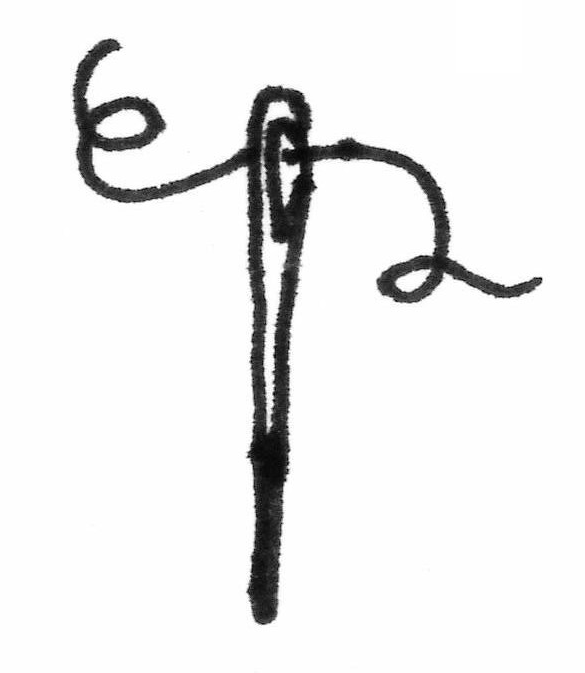
\includegraphics[scale=0.15]{../illustrations/thread}
\end{center}
\vspace{-1em}
\end{wrapfigure}
\fi

The rule {\sc E-Freeze-Final} detects quiescence by checking that two
properties hold.  First, every event of interest (lattice element in
$Q$) that has occurred (is bounded by the current LVar state) must be
handled (be in $H$).  Second, all existing callback threads must have
terminated with a value.  In other words, every enabled callback has
completed.  When such a quiescent state is detected, {\sc
  E-Freeze-Final} freezes the LVar's state.  Like {\sc
  E-Spawn-Handler}, the rule can fire at any time,
nondeterministically, that the handler appears quiescent---a transient
property!  But after being frozen, any further $\PUTi$ updates that
would have enabled additional callbacks will instead fault, causing
the program to step to $\error$.

Therefore, freezing is a way of ``betting'' that once a collection of
callbacks have completed, no further updates that change the LVar's
value will occur.  For a given run of a program, either all updates to
an LVar arrive before it has been frozen, in which case the value
returned by $\FAW$ is the lub of those values, or some update arrives
after the LVar has been frozen, in which case the program will fault.
And thus we have arrived at \emph{quasi-determinism}: a program will
always either evaluate to the same answer or it will fault.

To ensure that we will win our bet, we need to guarantee that
quiescence is a \emph{permanent} state, rather than a transient
one---that is, we need to perform all updates either prior to $\FAW$,
or by the callback function within it (as will be the case for
fixpoint computations).  In practice, freezing is usually the very
last step of an algorithm, permitting its result to be extracted. As
we will see in
Section~\ref{subsection:lvish-regaining-full-determinism-with-runparthenfreeze},
our LVish library provides a special @runParThenFreeze@ function that
does so, and thereby guarantees full determinism.
